\documentclass[a4paper]{article}
\usepackage[english]{babel}
\usepackage[a4paper,top=2cm,bottom=2cm,left=2cm,right=2cm,marginparwidth=1.75cm]{geometry}
\usepackage{amsmath}
\usepackage{amsfonts}
% \usepackage{amsthm}
\usepackage{amssymb}
\usepackage{graphicx}
\usepackage[colorinlistoftodos]{todonotes}
\usepackage[colorlinks=true, allcolors=blue]{hyperref}
\usepackage{import}
\usepackage{pdfpages}
\usepackage{transparent}
\usepackage{xcolor}
\usepackage{algorithmicx}
\usepackage{algpseudocode}

\usepackage{thmtools}
\usepackage{enumitem}
\usepackage[framemethod=TikZ]{mdframed}

\usepackage{xpatch}

\usepackage{boites}
\makeatletter
\xpatchcmd{\endmdframed}
{\aftergroup\endmdf@trivlist\color@endgroup}
{\endmdf@trivlist\color@endgroup\@doendpe}
{}{}
\makeatother

%\usepackage[poster]{tcolorbox}
%\allowdisplaybreaks
%\sloppy

\usepackage[many]{tcolorbox}

\xpatchcmd{\proof}{\itshape}{\bfseries\itshape}{}{}

% to set box separation
\setlength{\fboxsep}{0.8em}
\def\breakboxskip{7pt}
\def\breakboxparindent{0em}

\newenvironment{proof}{\begin{breakbox}\textit{Proof.}}{\hfill$\square$\end{breakbox}}
\newenvironment{ans}{\begin{breakbox}\textit{Answer.}}{\end{breakbox}}
\newenvironment{soln}{\begin{breakbox}\textit{Solution.}}{\end{breakbox}}

% \tcolorboxenvironment{proof}{
%     blanker,
%     before skip=\topsep,
%     after skip=\topsep,
%     borderline={0.4pt}{0.4pt}{black},
%     breakable,
%     left=12pt,
%     right=12pt,
%     top=12pt,
%     bottom=12pt,
% }
% 
% \tcolorboxenvironment{ans}{
%     blanker,
%     before skip=\topsep,
%     after skip=\topsep,
%     borderline={0.4pt}{0.4pt}{black},
%     breakable,
%     left=12pt,
%     right=12pt,
% }

\mdfdefinestyle{enclosed}{
    linecolor=black
    ,backgroundcolor=none
    ,apptotikzsetting={\tikzset{mdfbackground/.append style={fill=gray!100,fill opacity=.3}}}
    ,frametitlefont=\sffamily\bfseries\color{black}
    ,splittopskip=.5cm
    ,frametitlebelowskip=.0cm
    ,topline=true
    ,bottomline=true
    ,rightline=true
    ,leftline=true
    ,leftmargin=0.01cm
    ,linewidth=0.02cm
    ,skipabove=0.01cm
    ,innerbottommargin=0.1cm
    ,skipbelow=0.1cm
}

\mdfsetup{%
    middlelinecolor=black,
    middlelinewidth=1pt,
roundcorner=4pt}

\setlength{\parindent}{0pt}

\mdtheorem[style=enclosed]{theorem}{Theorem}
\mdtheorem[style=enclosed]{lemma}{Lemma}[theorem]
\mdtheorem[style=enclosed]{claim}{Claim}[theorem]
\mdtheorem[style=enclosed]{ques}{Question}
\mdtheorem[style=enclosed]{defn}{Definition}
\mdtheorem[style=enclosed]{notn}{Notation}
\mdtheorem[style=enclosed]{obs}{Observation}
\mdtheorem[style=enclosed]{eg}{Example}
\mdtheorem[style=enclosed]{cor}{Corollary}
\mdtheorem[style=enclosed]{note}{Note}

% \let\thetheorem=\relax
% \let\thelemma=\relax
% \let\theclaim=\relax
% \let\theques=\relax
% \let\thedefn=\relax
% \let\thenotn=\relax
% \let\theobs=\relax
% \let\thecor=\relax
% \let\thenote=\relax

% \renewcommand\qedsymbol{$\blacksquare$}
\newcommand{\nl}{\vspace{0.2cm}\\}
\newcommand{\mc}{\mathcal}
\newcommand{\mi}{\mathit}
\newcommand{\mf}{\mathbf}
\newcommand{\mb}{\mathbb}
\renewcommand{\L}{\mc{L}}
\newcommand{\hd}{\hat{\delta}}

\newcommand{\incfig}[1]{%
    \def\svgwidth{\columnwidth}
    \import{./figures/}{#1.pdf_tex}
}
\pdfsuppresswarningpagegroup=1

\title{\textbf{COL331 Assignment 2}}
\author{Navneel Singhal}
\date{}

\begin{document}
\maketitle
\tableofcontents

\section{Description}

The task assigned for this assignment was to write a multithreaded program that outputs all prime numbers upto some natural number $N$, using $t$ threads, using the Sieve of Eratosthenes.

\section{Running instructions}

The program is intended to be run using the following two ways.

\begin{enumerate}
    \item running \texttt{make} in the submission root directory -- this runs the program on $N = 10^6, t = 10$.
    \item running \texttt{make N=N\_0 t=t\_0} where $N_0, t_0$ are the values of $N$ and $t$ that are required to be used for the program.
\end{enumerate}

\section{Outputs}

The outputs from the run on my system are in the directory \texttt{output/local\_outputs/}.\nl
The outputs that are generated from the algorithm are:

\begin{enumerate}
    \item The timing statistics -- these are stored in a text file called \texttt{timing\_stats.txt} in the \texttt{output} directory.
    \item The primes generated as a result of running the algorithm -- this is stored in a text file called \texttt{primes.txt} in the \texttt{output} directory.
    \item The plot for the time taken for each thread (plotted as a clustered bar graph for each thread for both the approaches) -- this is shown at the end of the run, as well as stored in an
        image file called \texttt{timing\_plot.png} in the \texttt{output} directory. 
    \item The data file that is used by \texttt{gnuplot} to generate the plot -- this is stored in \texttt{stats\_for\_plotting.dat}.
\end{enumerate}

\section{Algorithm}

As per the specifications, there are two approaches. Both approaches use the segmented Sieve of Eratosthenes, which is as described in the Appendix.

Note that to avoid acquiring and releasing of mutexes too many times, we break the whole partition into small chunks of size $c$. This has been done uniformly across both approaches to ensure
there is as less difference in the implementation of both the approaches as possible, to get the best results.

\subsection{Na\"ive approach}

In this approach, we statically divided the first $N$ natural numbers into $t$ contiguous partitions, and ran the segmented sieve on each partition on a thread of its own. In the
implementation, this was done by grouping together contiguous \textit{chunks} (as described above), and processing those chunks in order with minimal overhead, so that each thread has roughly
$\lfloor N/t \rfloor$ integers that it needs to process.

\subsection{Load-balanced approach}

In this approach, we bring in load balancing by invoking a function called \texttt{allocate\_chunk} that maintains an internal counter which keeps track of the last chunk that was
allocated to a thread, and allocates a new chunk whenever it is called. The internal counter is the only data location that is ever written to by more than one thread, so we use one mutex that
guards the call of this function in a thread. In other words, exactly one thread can call this function at a time, so it is guaranteed that the chunk number returned (and updated) by the function
is indeed the correct value, and that it isn't garbled by two threads trying to change it at the same time.

\section{Brief implementation details}

\subsection{Algorithm details}

The high level description of the na\"ive algorithm is as follows:

\begin{enumerate}
    \item Precompute a sieve on the first $\sqrt{N}$ numbers.
    \item Divide the first $N$ natural numbers into chunks of size $c$.
    \item For each thread, run a function that takes the thread number, and using that, it takes a partition of the first $N$ natural numbers consisting of several chunks of size $c$, and
        generates primes for those chunks. Note that the primes are stored per chunk.
    \item Stitch together all these primes while outputting them.
\end{enumerate}

The high level description of the load-balanced algorithm is as follows:
\begin{enumerate}
    \item Precompute a sieve on the first $\sqrt{N}$ numbers.
    \item Divide the first $N$ natural numbers into chunks of size $c$.
    \item For each thread, run a function that calls the chunk allocator and for each chunk, runs the algorithm on that chunk, and stops when the chunk allocator runs out of chunks to give.
    \item Stitch together all these primes while outputting them.
\end{enumerate}

To reduce the memory requirements of the algorithm, I did some optimizations as follows:

\begin{enumerate}
    \item Allocate $O(c)$ memory for each chunk's sieve, leading to a total of $O(tc)$ memory usage for the segmented sieve part.
    \item Allocate $O(\sqrt{n})$ memory for the precomputation sieve.
    \item Implement a vector library to ensure that the total memory allocated for storing primes remains linear in the number of primes (which is $O(N / \log N)$). The actual memory for storing
        is this plus $O(N/c)$, since I had a vector pointer for each chunk.
\end{enumerate}

\subsection{Measurements}

There were two measurements that were carried out:

\begin{enumerate}
    \item Wall clock time -- This represents the time difference between the instances in time when the thread started running and when it ended running.
    \item CPU thread time -- This represents the time taken by the thread actively on the CPU, and excludes sleep time.
\end{enumerate}

The time that was actually used was CPU thread time, since it gives a better measure of the time taken by a thread in actually processing the data and hence is ideal for measuring the load
imbalance among threads.

\section{Parameters}

There were a few parameters that were used in the assignment.

\begin{enumerate}
    \item $N$: This was as given to us in the assignment $10^6$.
    \item $t$: This was the number of threads, as given to us in the assignment, with a default value of $10$.
    \item $c$: I experimented with chunk sizes in $\mc{O}(\sqrt{N})$, $\mc{O}(\sqrt[3]{N})$, and chunk sizes of various constant sizes. The most consistent results came
        from chunk sizes in $\mc{O}(\sqrt[3]{N})$, while for very large $N$ ($N \sim 10^8 - 10^{10}$), better performance for the load balanced version comes from chunk sizes in $\mc{O}(\sqrt{N})$. This is because mutexes
        might be slow and consequently the bottleneck in the program.
    \item Small primes: We needed to precompute the primes not exceeding $\sqrt{N}$, so this gives rise to a fixed parameter corresponding to each $N$ which breaks the set of primes not
        exceeding $N$ into two sets -- ``small" and ``big".
\end{enumerate}

\section{Results}

The plot of time taken per thread is as follows.

\begin{center}
    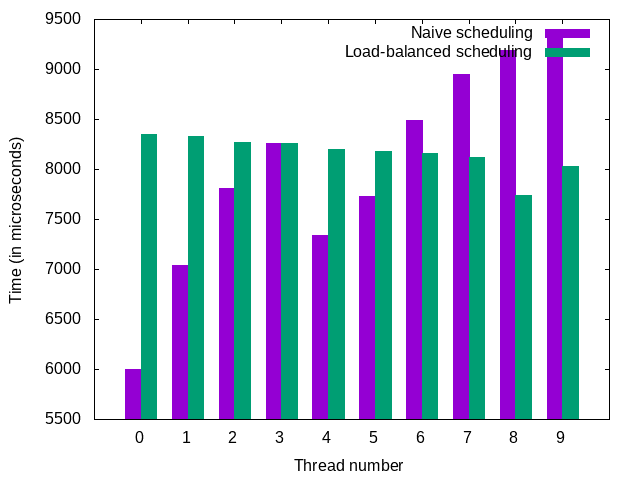
\includegraphics[scale=0.7]{./output/local_outputs/timing_plot.png}
\end{center}

From here, we note that there is a great deal of irregularity among the time taken for various threads in the na\"ive implementation, however the variation is quite low for the implementation
that does load scheduling of chunks.\nl

Some statistics from the set of primes obtained:

\begin{enumerate}
    \item There are 78498 primes below $10^6$.
    \item The largest prime not exceeding $10^6$ is $999983$.
\end{enumerate}

\section{Analysis}

From the plots, it seems like there is load balancing in the second approach, while there is no such balancing in the first approach. The reason behind this observation is two-fold.

\begin{enumerate}
    \item There is no load balancing in the first approach, since we are statically assigning chunks to threads, without paying
        heed to the fact that some threads end executing before other threads, and that they stay idle for the remaining time.
    \item In the second approach, threads can ask the chunk allocator to allocate more chunks to them, and hence actively try to not stay idle (apart from the time when there is another thread
        asking the chunk allocator to allocate more chunks to it, where it needs to wait till the allocator can allocate a chunk to it). Since the chunk ``computation" sizes are relatively small (and
        the number of chunks is large), the result of such a competition between threads is in fact the threads doing roughly equal amounts of work (more precisely, if the computation time for a
        chunk is upper bounded by $T$ (and the allocation time is negligible compared to this), then there is no pair of threads whose end time differs by more than $T$.
\end{enumerate}

\section{Appendix -- Segmented Sieve of Eratosthenes}

The idea behind the segmented sieve of Eratosthenes is mainly the following.\nl
Consider any natural number $n$. If it is composite, then $n = ab$ for some $1 < a \le b < n$, with $a, b \in \mb{N}$. Hence we have $a \le \sqrt{N}$. Hence, if we precompute all primes from $1$ to
$\sqrt{N}$, then we will only need to check all numbers from $1$ to $n$ for being divisible by a prime in this set.\nl
We proceed to the present a modification of the sieve of Eratosthenes, where we consider numbers in a range $[l, r]$. In the simple sieve of Eratosthenes, a prime $p \le
\lfloor\sqrt{N}\rfloor$ strikes out the numbers $p^2, p^2 + p, \ldots, p\lfloor\frac{N}{p}\rfloor$. Hence in this range, it will strike out the numbers in the intersection of this set with $[l, r]$. When the sum is taken over the union of
all such ranges, the number of steps taken is the same as number of steps taken in the sieve of Eratosthenes (apart from a few book-keeping steps to find the starting point etc.). This forms the
basis of the segmented sieve of Eratosthenes. The number of steps taken in processing one chunk $[l, r]$ is upper bounded by $r - l + 1$ times the sum of reciprocals of primes $\le \sqrt{N}$, which
using the prime number theorem is in $O((r - l + 1) \cdot \log \log n)$.

\end{document}
